\documentclass{jsarticle}
\usepackage[dvipdfmx]{graphicx}
\begin{document}

\title{身体動作と筋電量の関係性}
\author{平松亨隆}
\maketitle


\section{目的}
私を含めて人は、体を動かすときに意識的に筋肉の伸縮を考えて体を動かすわけではない。だから、例えば腕を曲げるときに上腕二頭筋をどれくらい収縮させるかなどと考える人はいないだろう。そこで、どのように筋肉を収縮させて運動しているのかということを本レポートの目的とした。

\section{実験方法}
\subsection{運動計測}
下記の図\ref{fig:short}はもっとも腕を曲げた状態、図\ref{fig:long}は最も腕を伸ばした状態の図である。被験者にはこの2つの状態を繰り返す腕の曲げ伸ばし運動を、何も指示を出していない速度と速い速度の2パターンで利き腕を動かしてもらって計測をした。被験者には反射マーカーを肩、肘、手首につけて。また筋電センサ(ロジカルプロダクト社)を上腕二頭筋と上腕三頭筋に貼付し、筋電位をサンプリング周波数は200 Hzで計測した。筋電センサとカメラの計測時間は同期をとり、20秒間計測していた。
\begin{figure}[h]
  \begin{minipage}{0.5\hsize}
    \begin{center}
      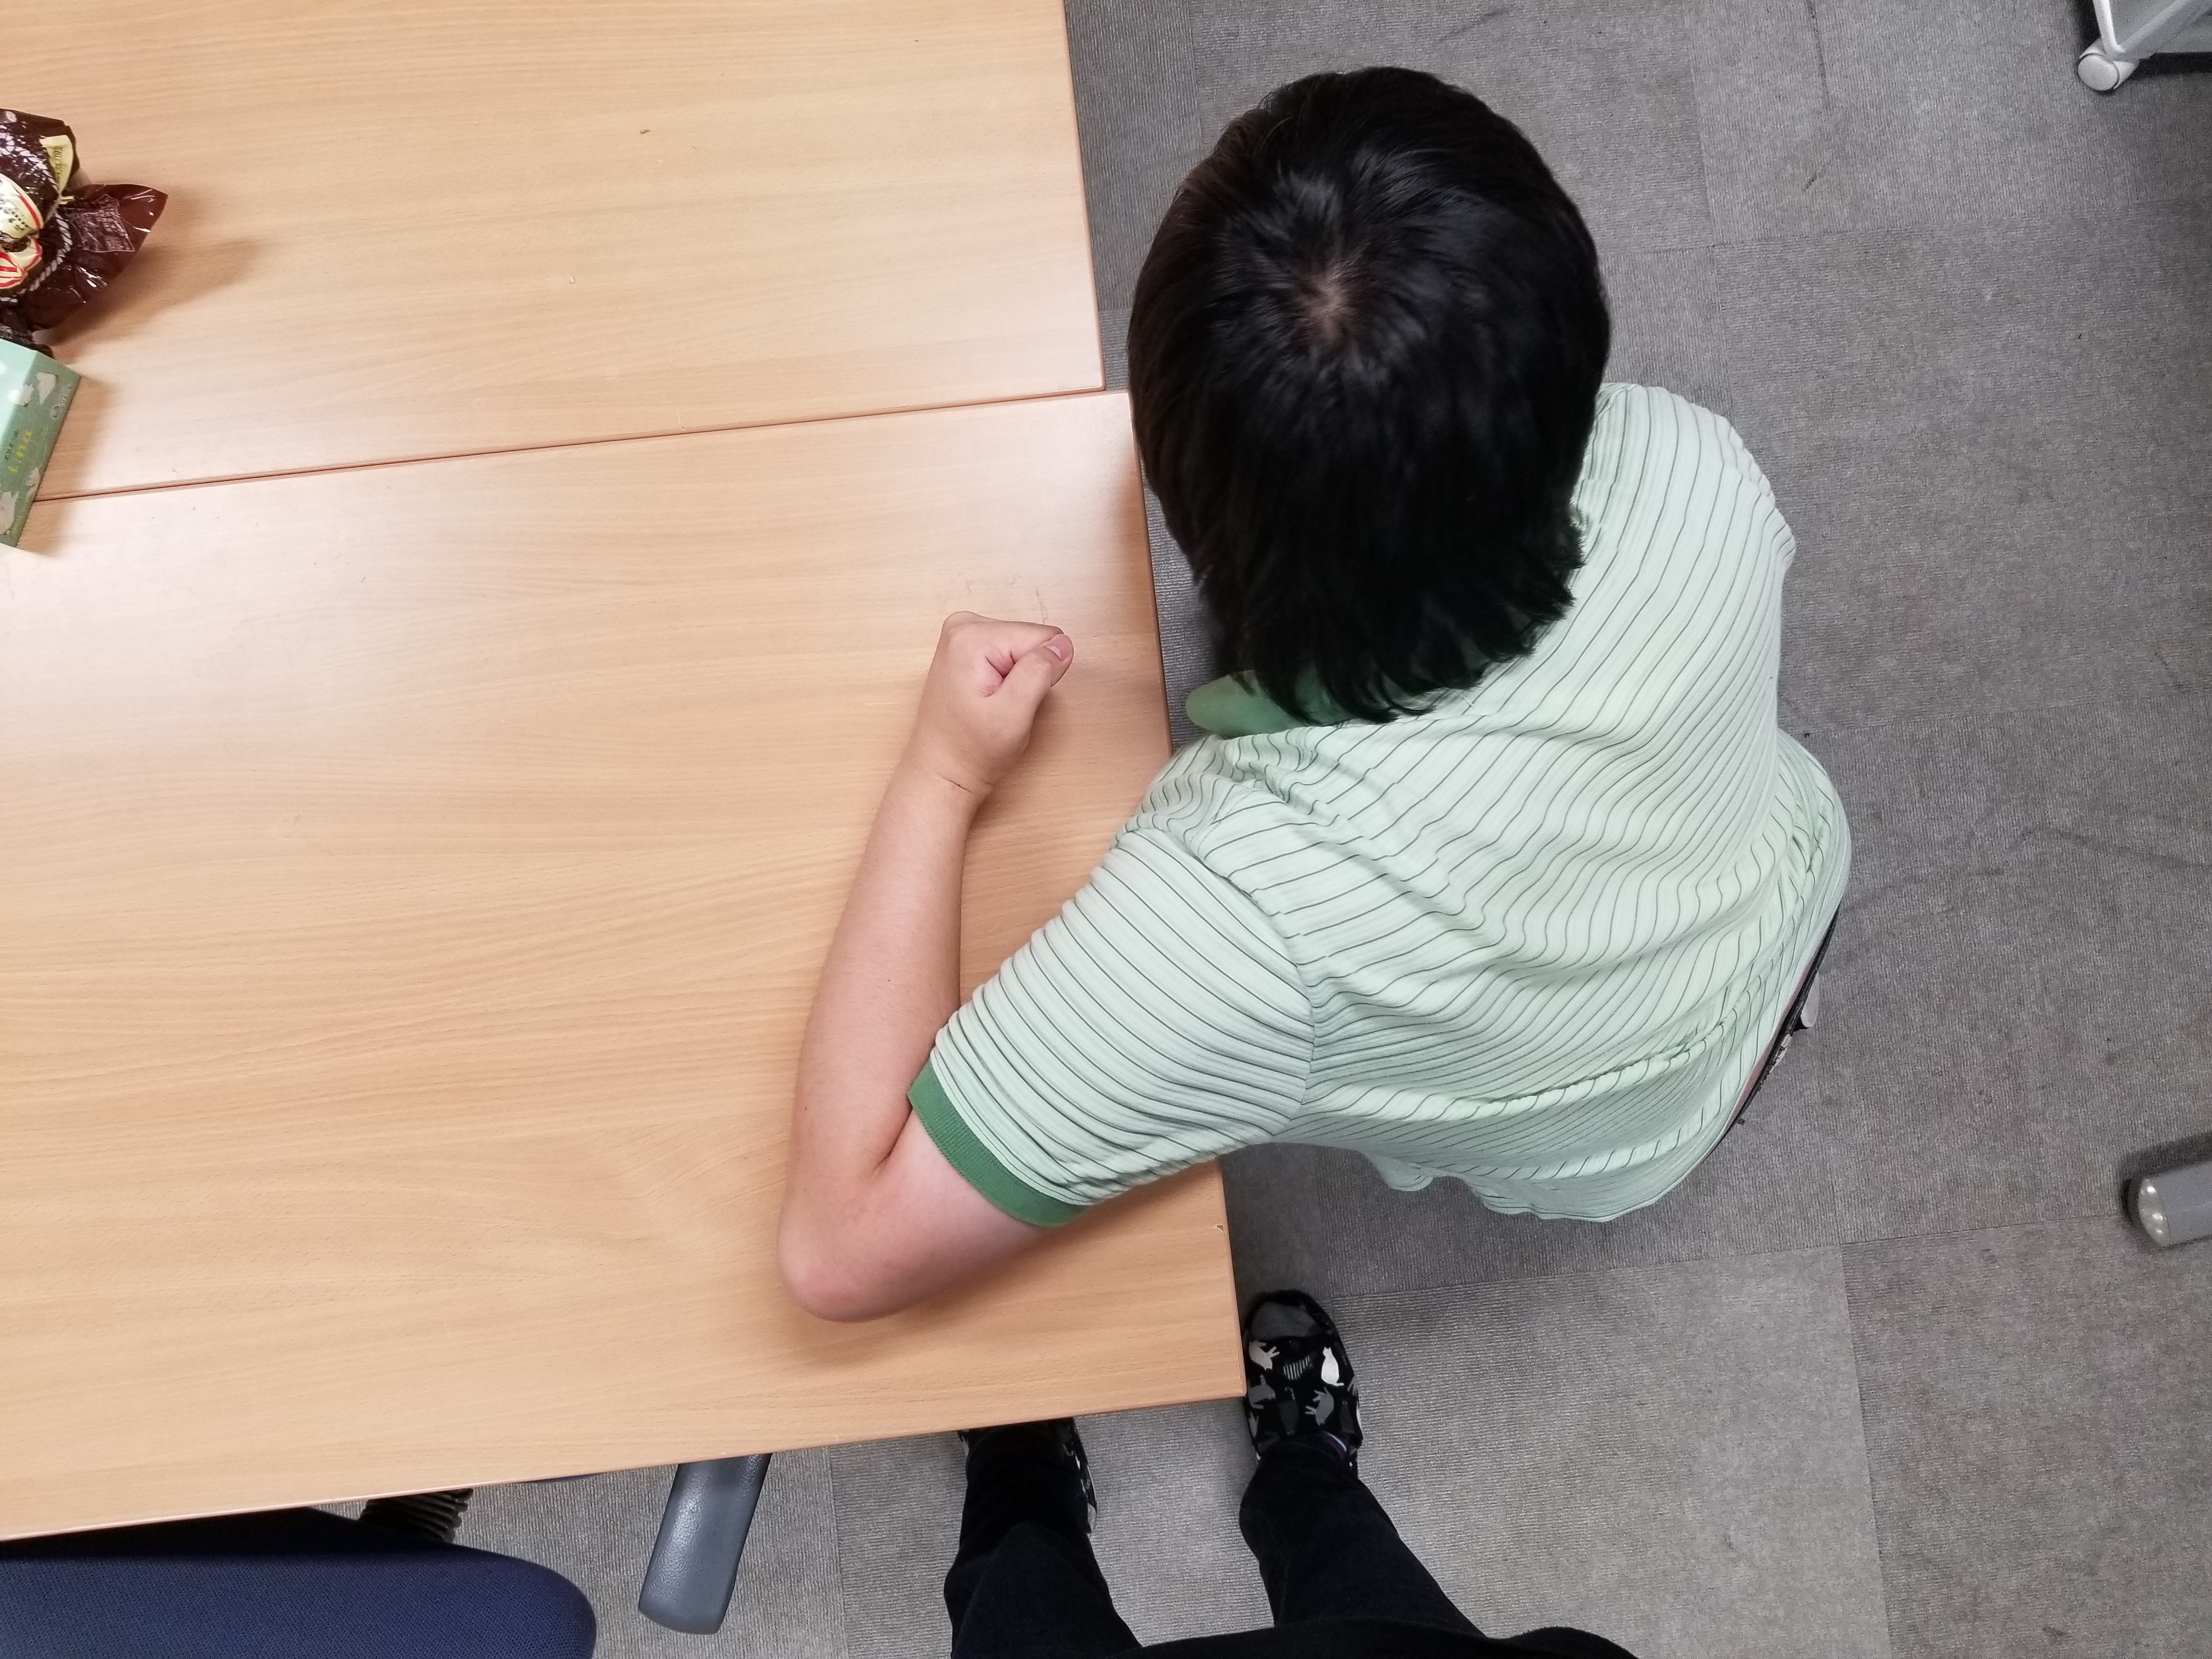
\includegraphics[width=7cm]{images/short.jpg}
    \end{center}
    \caption{腕を縮めた状態}
    \label{fig:short}
  \end{minipage}
  \begin{minipage}{0.5\hsize}
    \begin{center}
      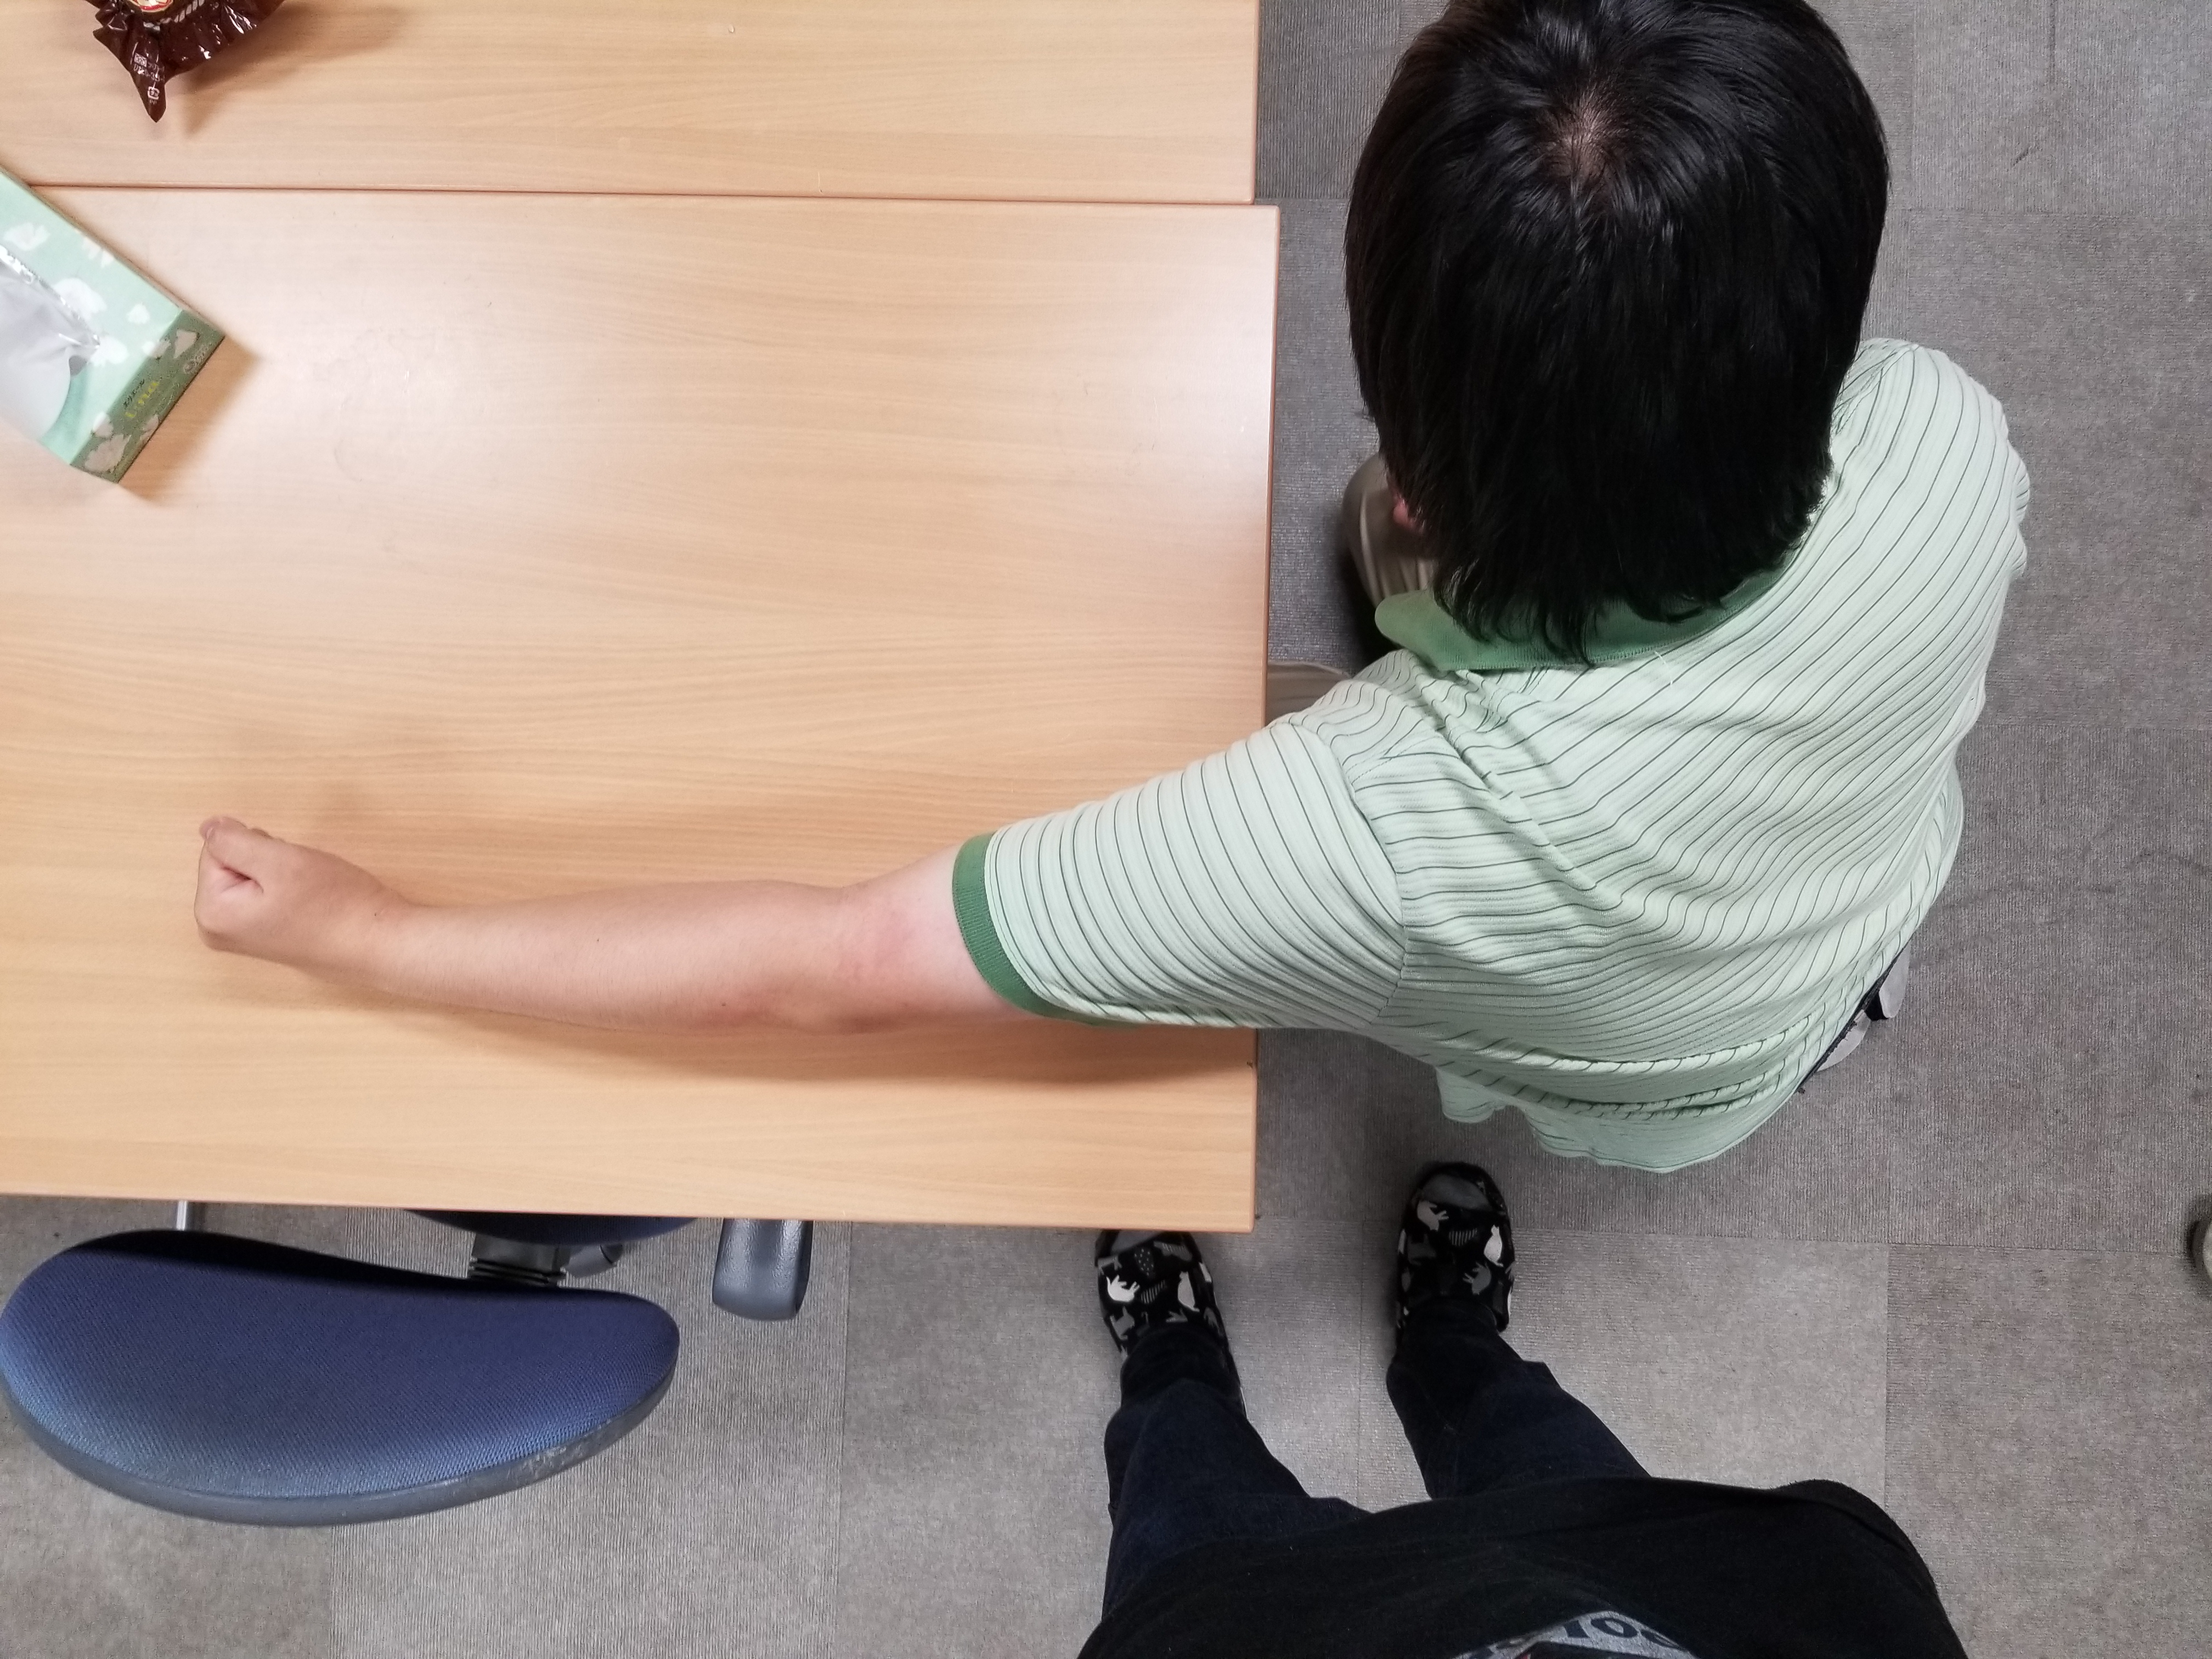
\includegraphics[width=7cm]{images/long.jpg}
    \end{center}
    \caption{腕を伸ばした状態}
    \label{fig:long}
  \end{minipage}
\end{figure}

\subsection{解析}
\subsubsection{筋電位}
筋電位のデータにはいくつかの処理を順番に施して、筋肉の活動度を求めた。
  まずデータから筋電位の特徴を抽出するために、通過帯域を1〜40 Hzとしたバンドパスフィルタ(3次バターワース)をかけた。しかし、バンドパスフィルタをかけることによってデータに位相ズレが生じるため、時間軸を反転してもう一度同じフィルタをかけることによってこれを補正した。そしてフィルタ後のデータに整流し、時刻$t$の筋電位$|E(t)|$を$\Delta T$の間で平均を求め、筋肉の活動度とした。式は以下のものを用いた。
  \begin{equation}
    a(t) = \frac{1}{\Delta T} \int_{t-\frac{\Delta T}{2}}^{t+\frac{\Delta T}{2}} |E(t)| dt
  \end{equation}

\section{結果}
\begin{figure}[h]
  \begin{center}
    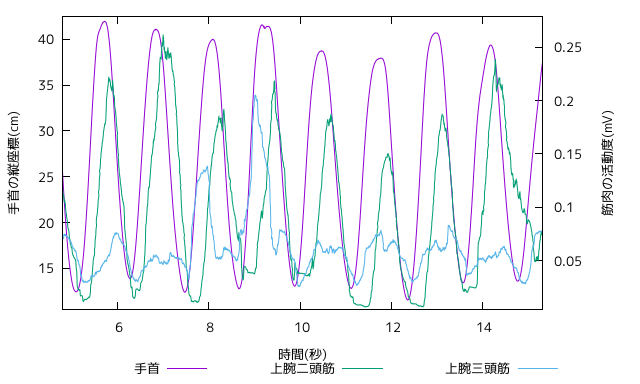
\includegraphics[width=15cm]{images/s1proto.png}
  \end{center}
  \caption{スロー時の運動と筋肉の活動度の関係}
  \label{fig:slow}
\end{figure}
図\ref{fig:slow}は、特に指示を出さず腕を動かしてもらった時である。身体に対する手首の前後方向の変位と筋肉の活動度を縦軸に、そして時間を横軸とした。このとき身体に対する手首の前後方向の変位は、体の前に伸ばすほど値は大きくなる。図中の紫、緑、青の線はそれぞれ身体に対する手首の前後方向の変位、上腕二頭筋肉の活動度、上腕三頭筋の活動度である。手首の前後方向の変位が、横方向や縦方向に比べて変位が大きく、動きが把握しやすい部分であったので抜き出した。このグラフでは、見やすくするために時刻5〜15秒の間を拡大表示している。

図\ref{fig:slow}から、例えば時刻10秒の時、腕がもっとも曲げられた状態で伸ばされ始め、少ししてから上腕二頭筋の活動度が大きくなっていっている。そして、伸ばしきったあとある程度腕を曲げたところでその活動度を下げはじめている。これはほとんどの場合において言えることである。またこの時上腕三頭筋は、最大値が上腕二頭筋よりもかなり小さいが、同じような挙動をしている。しかし、いくつかの例においては、腕を伸ばし始めてから伸ばしきるまでの間だけ、上腕二頭筋に匹敵する活動度を見せているものもある。

\begin{figure}[h]
  \begin{center}
    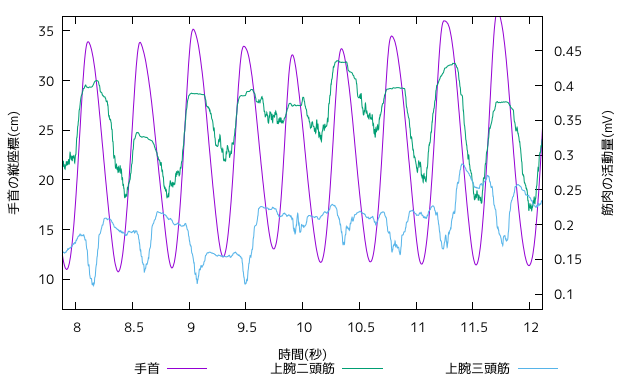
\includegraphics[width=15cm]{images/s2proto.png}
  \end{center}
  \caption{スロー時の運動と筋肉の活動度の関係}
  \label{fig:fast}
\end{figure}
図\ref{fig:fast}は、腕を速く動かしてもらった時のものである。軸や凡例は図\ref{fig:slow}と同様である。図\ref{fig:fast}から、例えば時刻8.8秒の時、腕がもっとも曲げられた状態では上腕二頭筋の活動度は低い、この状態から腕が伸ばされ始めると同時に活動度が大きくなっていっている。また腕を曲げるにしたがってその活動度を下げている。要するに手首の前後方向の変位と似たような形である。このとき上腕三頭筋は、腕をもっとも曲げた状態では活動度が大きく、腕が伸ばされるにしたがってその値が小さくなっていっている。これは、上腕二頭筋の逆位相のような形である。

図\ref{fig:slow}と図\ref{fig:fast}を比較すると、速度が違うだけの同じ運動で、図\ref{fig:slow}では上腕二頭筋と上腕三頭筋の活動度ではほぼ同じ位相、図\ref{fig:fast}では逆位相、となっている。また、図\ref{fig:slow}では上腕二頭筋と上腕三頭筋の活動度の最低値が近いのに対し、図\ref{fig:fast}では最低値が大きく離れている。
\section{考察}
結果で触れた上腕二頭筋と上腕三頭筋の活動度の速度による位相差はなぜ起きたのか。これは、上腕二頭筋と上腕三頭筋の発達度の違いによって生じた可能性がある。基本的に二頭筋は三頭筋より発達している。自然に動かすときは筋肉はそれほどの活動度を示さないはずだが、二頭筋は三頭筋よりも高い活動度を示すために、三頭筋は二頭筋をブレーキのように抑える必要が出てくる。また三頭筋はあまり発達していないため、腕を伸ばすときは活動度がほとんど上がらない。これらによって、自然に動かすときは起伏の位置が同じになっているのではないだろうか。

このことから、人は体を動かすときに上腕二頭筋と上腕三頭筋のような逆の働きをする筋肉をアクセルとブレーキのように使い分けて体を操作しているのではないかとも言える。例えば腕を速く動かすときは上腕二頭筋も上腕三頭筋もそれなりの活動度を要求されるため、腕を伸ばすときは上腕二頭筋がブレーキで上腕三頭筋がアクセル、腕を曲げるときは上腕二頭筋がアクセルで上腕三頭筋がブレーキ、というように役割を切り替えて活動してるのだろう。そのために、図\ref{fig:fast}は筋活動度が逆位相になっている。
\end{document}